\documentclass[10pt]{article}
\usepackage[final]{graphicx}
\usepackage{amsfonts}

\topmargin -.5in
\textwidth 6.6in
\textheight 9in
\oddsidemargin 0in
\usepackage{color}
\newcommand{\arvind}[1]{{\color{red}{Arvind: {#1}}}}

\def\ds{\displaystyle}
\def\d{\partial}

\begin{document}

\centerline{\large \bf Fusing surface and satellite-derived PM observations to determine the impact } 

\centerline{\large \bf of international transport on coastal PM$_{2.5}$ concentrations in the western U.S.}

\vspace{.1truein}

\def\thefootnote{\arabic{footnote}}
\begin{center}
  Neha Bora\footnote{Department of Mathematics, Iowa State University},
  Tuo Chen\footnote{Department of Statistics, University of Florida},
  Dana Cochran\footnote{Department of Mathematics, California State University Channel Islands},
  Kelly Dougan\footnote{Department of Mathematics, The State University of New York at Buffalo},
  Gautam Sabnis\footnote{Department of Statistics, Florida State University}
  Chuanping Yu \footnote{Industrial and System Engineering, Georgia Institute of Technology}
\end{center}

%\vspace{.1truein}

\begin{center}
Faculty Mentors: mentor 1\footnote{Company},
Mentor 2\footnote{University}
\end{center}


\vspace{.3truein}
\centerline{\bf Abstract}

Long term exposure to PM$_{2.5}$ is associated with human health complications (insert citation). Surface readings of PM$_{2.5}$ in the states on the West Coast of the United States have reported to be higher than allowed by the Clean Air Act. One possible reason for this is international transport of air pollution on PM$_{2.5}$. This project explores the relationship between the surface readings of PM$_{2.5}$ from coastal sites with the AOD measurements from the AVHRR in these regions. Once we found a correlation between these readings, we implemented a model to approximate PM$_{2.5}$ concentrations in the Pacific ocean, where surface readings are not possible.

\section{Introduction}
\arvind{This is not the right material to be covered in an introduction, so I have reorderded. The  introduction should roughly cover the following points
\begin{itemize}
\item A bird's eye view of the problem, i.e. adverse effect of pollution
\item Review of previous work and main findings (the three papers Brett sent)
\item What the main goals of this paper are (essentially paraphrasing Elizabeth's and Brett's goals). 
\item Our main contributions in this report. 
\end{itemize}
}

Domestic sources of emissions are the primary cause of air pollution in the U.S.; however, there is potential for international flow of air pollution into the U.S. to be a contributing factor in some coastal cities having high recorded measurements of air pollution. The impact that international transport of air pollution has on our ability to attain air quality standards or other environmental objectives in the U.S. has yet to be fully characterized. In other words, cities in the western U.S. may unknowingly be receiving high pollutant values through no fault to themselves. The goal in this project is to establish a connection between AOT measurements from the AVHRR satellite to determine the impact of international transport of air pollution on PM$_{2.5}$ concentrations in coastal areas of the western U.S. We examined PM$_{2.5}$ sites that were close to the coast. Most of our sites were situated in California, with a few in Washington and a handful in Hawaii. The map in figure 1 shows the 13 sites that were used along the Western U.S. coast. 



For this project, we used two different sources of data -- Aerosol Optical Thickness (AOT) obtained from satellite measurements, and surface PM$_{2.5}$ measurements. ~\arvind{Please explicitly define AOT. }
PM$_{2.5}$ is particulate matter that is less than $2.5$ micrometers in diameter and is often referred to as the greatest health risk of pollutants~\cite{epa}.

\section{The Problem}
%\begin{figure}[ht!]
%\centering
%\includegraphics[width = 90mm]{pmsites.jpg}
%\caption{}
%\label{graph3}
%\end{figure}


\subsection{Description of data}

The first data set of Climate Data Record (CDR) of AOT was obtained from by the National Oceanic and Atmospheric Administration (NOAA)~\cite{noaa}. This data was collected using the  Advanced Very High Resolution Radiometer (AVHRR) that provides an optical measure of aerosol column loading derived form the global ocean pixel-level PATMOS-x AVHRR clear-sky reflectance CDR at $0.63$ $\mu$m channel~\cite{noaa}. This satellite provides global readings of oceanic measurements of AOT on a daily, as well as a monthly scale, for the years $1981$-$2009$~\cite{noaa}.

The second data set consisting of the PM$_{2.5}$ measurements, was taken on land sites in California, Oregon, Washington, Alaska, and Hawaii. This was provided by the United States Environmental Protection Agency (EPA).   PM$_{2.5}$ is so small that it can get lodged into lungs and make it difficult for people to breath. This creates an increase in respiratory problems. Common contributing factors to PM$_{2.5}$ include emissions for motor vehicles, power plants, wood burning, and dust from paved or unpaved roads, \cite{epa}.

The AVHRR takes approximately $16$ days to cover the entire earth. We, thus, have roughly two data values for each month of the year. The frequency of the PM$_{2.5}$ data is variable and ranges from once every day to once every six days. On certain occassions, the measurements from the satellite were found to be  erroneous due to light reflection from cloud covers. Additionally, there are times when the PM$_{2.5}$ sensors malfunctioned resulting in no data. These points were appropriately removed from the datasets. Hence, we sometimes have months that have only two or less PM$_{2.5}$ data and/or no AOT data. 

\subsection{Challenges}
\arvind{Here I would list the challenges associated with the data, lack of spatial and temporal coverage, etc. The differences between what we would like to have vs what we have instead.}
\section{The Approach}

\subsection{Data processing}
\arvind{Describe what other preprocessing was done to the data.} 

%\subsubsection{Clean the AVHRR AOD data}

No matter what PM2.5 sites we use, we need to find the closest AOD coordinates to the PM2.5 sites, and then to match the sites data for each day. This requires us to search all the observations in AOD dataset. The AOD data are very large and we cannot put all the data in hundreds of files into one matrix. Besides, AOD data have lots of missing data. So we need to clean the AOD data first. 

Since the data we want to use are the data located on the west coast and Hawaii, first we used the longitude and latitude of the west coast and Hawaii to eliminate data from other locations that we won\rq t use. Then, we dropped all the missing data and also changed the original format of the data into more readable one. Finally, our AOD data looks like Table \ref{table3.1}. 

\subsection{PM$_{2.5}$ sites adjacent to AVHRR grids}
Since the coverage of the AOT data is over the oceans, and the PM$_{2.5}$ data is collected over the land, there is no direct overlap between the two datasets. In order to compare the two data sets, we adopt the following strategy. First, of all the PM$_{2.5}$ measurement sites, we identify those that are close to the coast. Figure~\ref{graph3} shows the geographical location of all the PM$_{2.5}$ sites, whereas Figure~\ref{graph4} shows the geographical locations to $13$ locations -- four of these are found in California, whereas the rest can be found in Hawaii.  In the rest of this report, we focus on only these $13$ locations. \arvind{Can you also mention that we only chose overlapping temporal data.}


%As AVHRR satellites can only get the aerosol optical depth (AOD) from oceans and PM$_{2.5}$ data are from lands, our strategy for identifying PM$_{2.5}$ sites is to choose the ones that are as close to the coast as possible.  The sites were chosen due to their proximity to the west coast. 

\begin{figure}[ht!]
\centering
\includegraphics[width = 90mm]{ALLPMsites.png}
\caption{\arvind{Please fill in the caption}}
\label{graph3}
\end{figure}




\begin{figure}[ht!]
\centering
\includegraphics[width = 90mm]{PMsites.png}
\caption{\arvind{The figure only shows the California locations, can the figure include the Hawaii sites as well? This map could also be zoomed in further. Also add a caption.}}
\label{graph4}
\end{figure}




\subsection{Analzing PM$_{2.5}$ trends}
One method we used to analyze trends in the PM$_{2.5}$ data was to make an animation to show the change in the concentration of PM$_{2.5}$  over time. The animation plots points at each site where the PM$_{2.5}$ data was collected, with color varying depending on the intensity of the reading, with darker colors indicating a larger concentration of PM$_{2.5}$. 

\arvind{Tuo: Please describe the time-series models you used to analyse PM data}


\arvind{The results of the experiments should be discussed in the next section}.
After analyzing this data we noticed (insert conclusion here... talk about it more...). The animation is available online (insert website-github?).

\subsection{Relationships between AVHRR AOD and surface PM$_{2.5}$}
We noticed that there was a huge difference between the  $13$ sites we identified along the West Coast and the sites located on Hawaii. The sites on Hawaii are unique because Hawaii is surrounded on water. Thus we decided to build models separately for both the sites along the West Coast and the sites on Hawaii. 

%\arvind{Yu: Describe the random effects model here. }

\subsubsection{Only AOD data}
Since there are many meteorological parameters varying from day to day, our statistical model must have the variability of the date. For each location, there are many different geographical properties, so our model must have the variability of sites. Therefore we used mixed effects model to fit this relationship:

$$PM_{ij} = \alpha + \beta\times AOD_{ij} + s_i + d_j+ \epsilon_{ij}, $$

where $PM_{ij}$ is the $PM_{2.5}$ concentration at a spatial site $i$ on a specific day $j$, $\alpha$ is the fixed intercept, $\beta$ is the fixed slope, $AOD_{ij}$ is the AOD value at a spatial site $i$ on a specific day $j$, $s_i\sim N(0, \sigma_s^2)$ is the random intercept of site $i$, $d_j\sim N(0, \sigma_d^2)$ is the random intercept of a specific day $j$, and $\epsilon_{ij}\sim N(0, \sigma^2)$ is the error term at site $i$ on a day $j$.

\subsubsection{AOD data and wind data}

\begin{table}[!h]
\centering
\begin{tabular}{|c|c|c|c|}
\hline 
Date & lat\_aot & long\_aot & aot\\
\hline
2000-01-25 & 30 & -126.6 & -0.0836133733391762 \\
\hline
$\cdots$ & $\cdots$ & $\cdots$ & $\cdots$\\
\hline
\end{tabular}
\caption{AOD data}
\label{table3.1}
\end{table}

\subsubsection{Match the AOD data with the PM2.5 data}
As we are trying to find the relationships between AOD and PM2.5, we need to keep all the date the same, and locations closest. After matching these two datasets, we got the following as in Table {table3.2}.

\begin{table}[!h]
\centering
\begin{tabular}{|c|c|c|c|c|c|c|}
\hline 
Date & lat\_pm & long\_pm & pm & lat\_aot & long\_aot & aot\\
\hline
2006-12-28 & 40.776944 & -124.1775 & 17.8 & 40.9 & -124.3 & 0.043815478682518\\
\hline
$\cdots$ & $\cdots$ & $\cdots$ & $\cdots$ & $\cdots$ & $\cdots$ & $\cdots$\\
\hline
\end{tabular}
\caption{AOD and PM2.5 match data}
\label{table3.2}
\end{table}





%%%%%%%%%%%%%
\section{Computational Experiments}
\arvind{I suggest organizing this section into a series of experiments. Here are a few suggestions. You can also follow the instructions at the end of the section.}

\subsection{Experiment 1: Analysis of PM25 time series}

\subsection{Experiment 2: PM 25 vs AOT data}
%%%%%%%%%%%%%%%%%%%%%%%%%%%%%%%%%%%%%%%
\subsubsection{Sites closest to the west coast}
If we only use the AOD data, by using the approach in Section ????, we fitted the mixed effects model as follows.

$$\hat{PM}_{ij} = 10.51 + 3.60\times AOD_{ij} + \hat{s}_i + \hat{d}_j, $$

where $\hat{s}_i\sim N(0, 1.79^2)$ and $\hat{d}_j\sim N(0, 3.04^2)$. 

The correlation between the fitted PM$_{2.5}$ data and the true PM$_{2.5}$ data is 0.802, which we agreed it is not a bad fit. 

If we use both the AOD data and the wind data, we built a multivariate linear regression model. As in Figure XXX, different sites have different relationships between AOD and PM. 

The following analysis is about the site (40.80178, -124.1621). For other sites, analysis should be similar. 

$$\hat{PM} = -0.64 - 0.0176\times AOD - 0.11\times WindSpeed + 0.45\times WindDirection + 0.017\times Humidity - 0.16\times AirTemp + Season + Year, $$

where Season and Year are factor variables. $R^2 = 0.758$.

\begin{figure}[ht!]
\centering
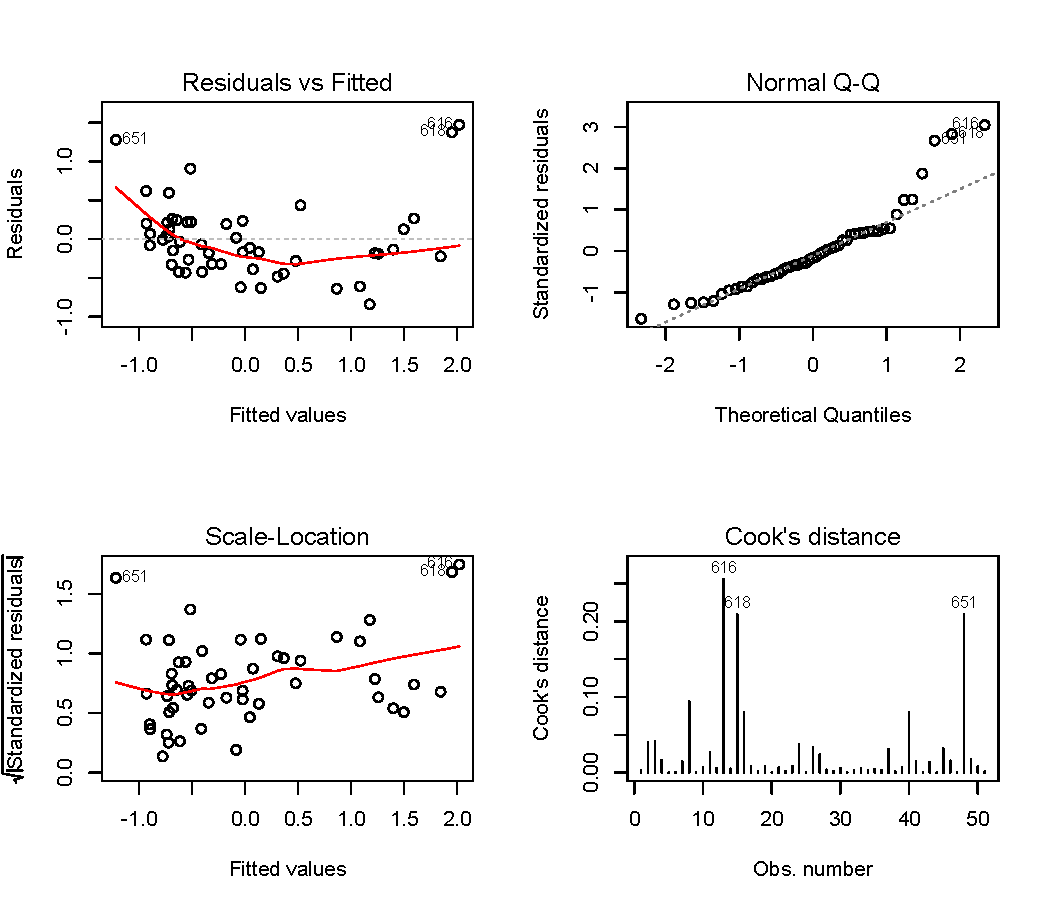
\includegraphics[width = 90mm]{residual.pdf}
\caption{}
\label{graph5}
\end{figure}

We can see from the above plots that there are three outliers. After deleting these outliers, the model became:

$$\hat{PM} = 94.43 + 2.34\times AOD - 1.11\times WindSpeed + 0.033\times WindDirection - 0.068\times Humidity - 0.30\times AirTemp + Season + Year, $$

where Season and Year are factor variables. $R^2 = 0.822$.

Then we did the stepwise to choose the best fit, we get the following model:

$$\hat{PM} = 3.42 -1.07\times WindSpeed + 0.036\times WindDirection + Season, $$
where Season is a factor variable. $R^2 = 0.786$.

\begin{figure}[ht!]
\centering
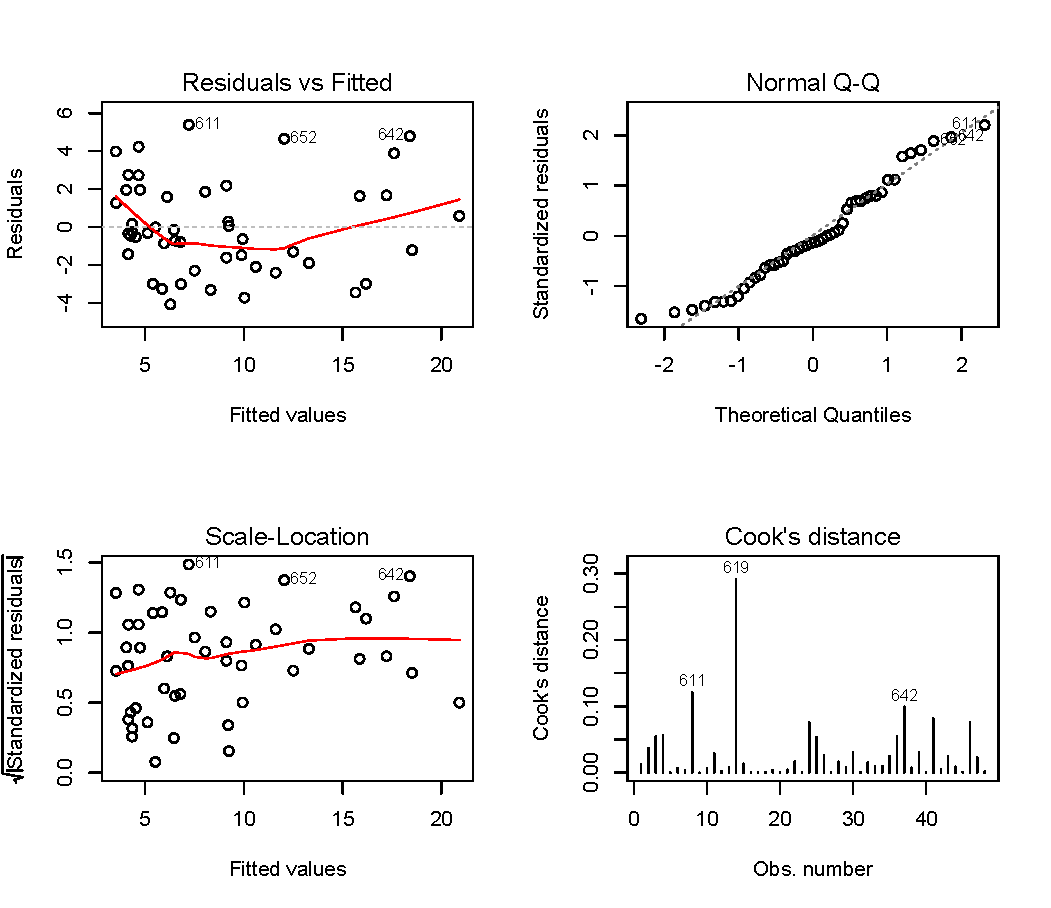
\includegraphics[width = 90mm]{residual2.pdf}
\caption{}
%\label{graph5}
\end{figure}

The results are better than the previous model. But we can see from those plots that the residuals still have some trend and some cluster. To figure out if this model is good, we did 5-folder cross validation. The results are as follows:

\begin{figure}[ht!]
\centering
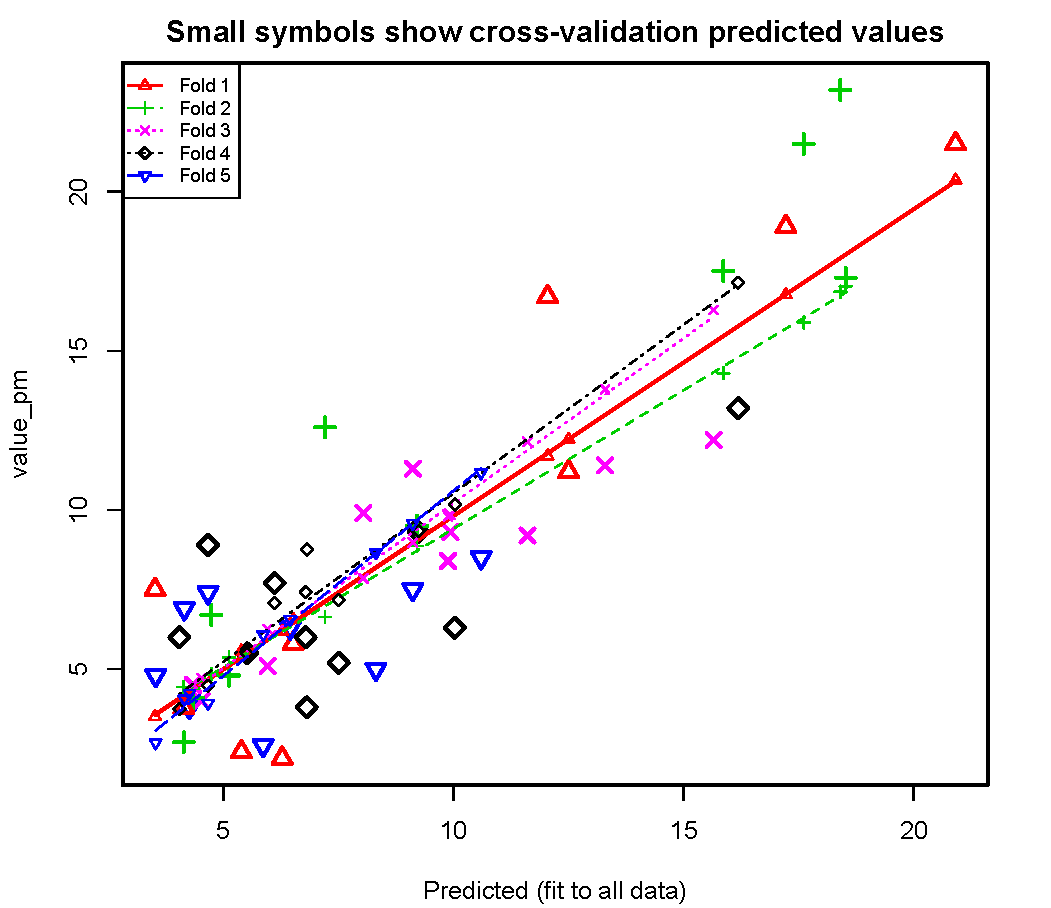
\includegraphics[width = 90mm]{cv_lm.pdf}
\caption{}
%\label{graph5}
\end{figure}

The mean square error is 8.16, which is very high due to the average PM values is 8.75. So multivariate linear regression is not a good model.

\subsubsection{Hawaii sites}
Similarly, we can get the mixed effects model for Hawaii sites.
Without the wind data,

$$\hat{PM}_{ij} = 6.205 + 7.780\times AOD_{ij} + \hat{s}_i + \hat{d}_j, $$

where $\hat{s}_i\sim N(0, 4.05^2)$ and $\hat{d}_j\sim N(0, 2.83^2)$. 

The correlation between the fitted PM$_{2.5}$ data and the true PM$_{2.5}$ data is 0.879, which is better than the west coast data. 

%%%%%%%%%%%%%%%%%%%%%%%%%%%%%%%%%%%%%%%%%




\subsubsection{relationships between AVHRR AOD and surface PM2.5 for sites closest to the west coast}

For sites closest to the west coast, we finally found 4 sites that have common date information. Figure \ref{fig3.3} is the plot regarding the AOD and PM2.5 by each site. 

\begin{figure}[!h]
\centering
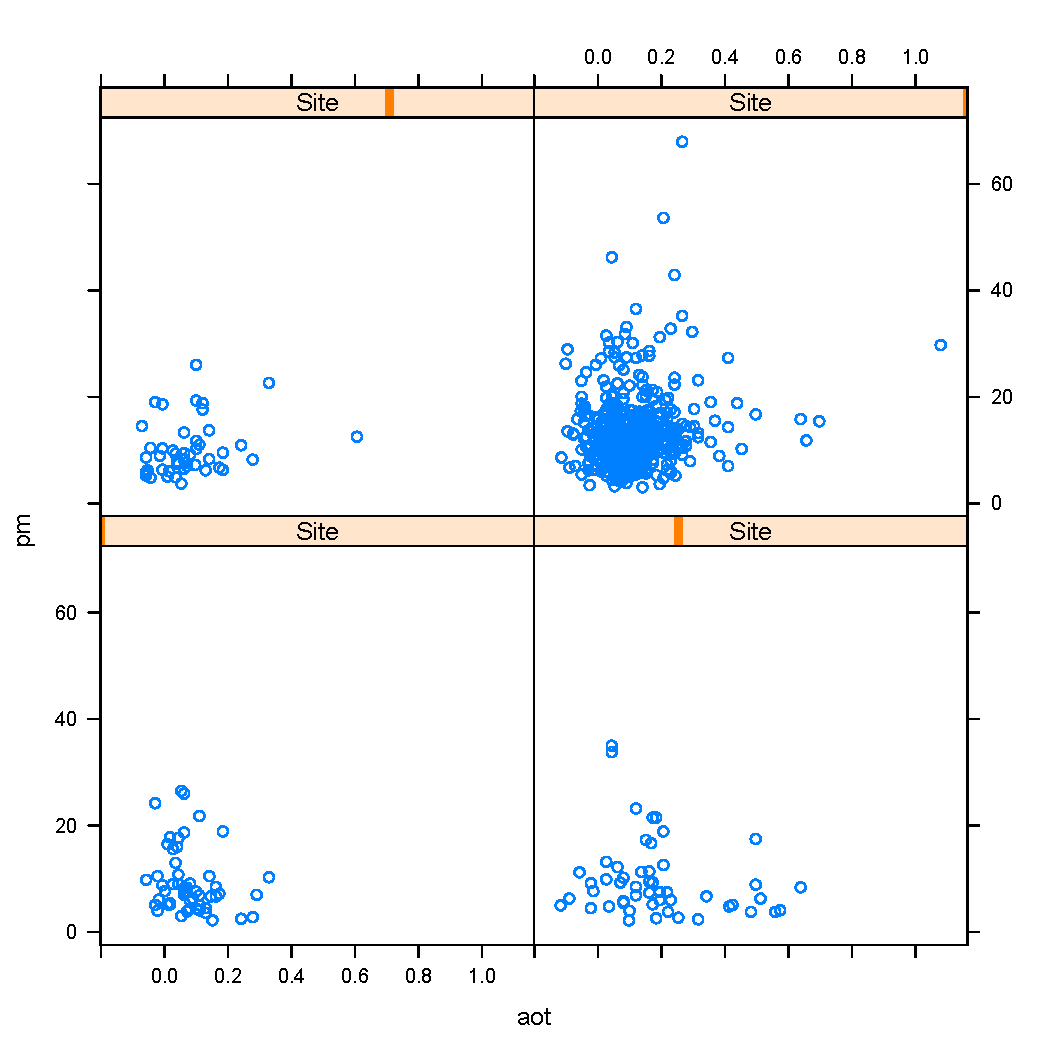
\includegraphics[width=\linewidth]{3.pdf}
\caption{PM vs. AOD for each site close to the west coast}
\label{fig3.3}
\end{figure}

We can see from the above plot that the relationships between AOD and PM2.5 are different for different sites. So we consider building different models for each site to find the relationships.

\subsubsection{relationships between AVHRR AOD and surface PM2.5 for Hawaii sites}

For Hawaii sites, we finally found 9 sites that have common date information. Figure \ref{fig3.4} is the plot regarding the AOD and PM2.5 by each site. 

\begin{figure}[!h]
\centering
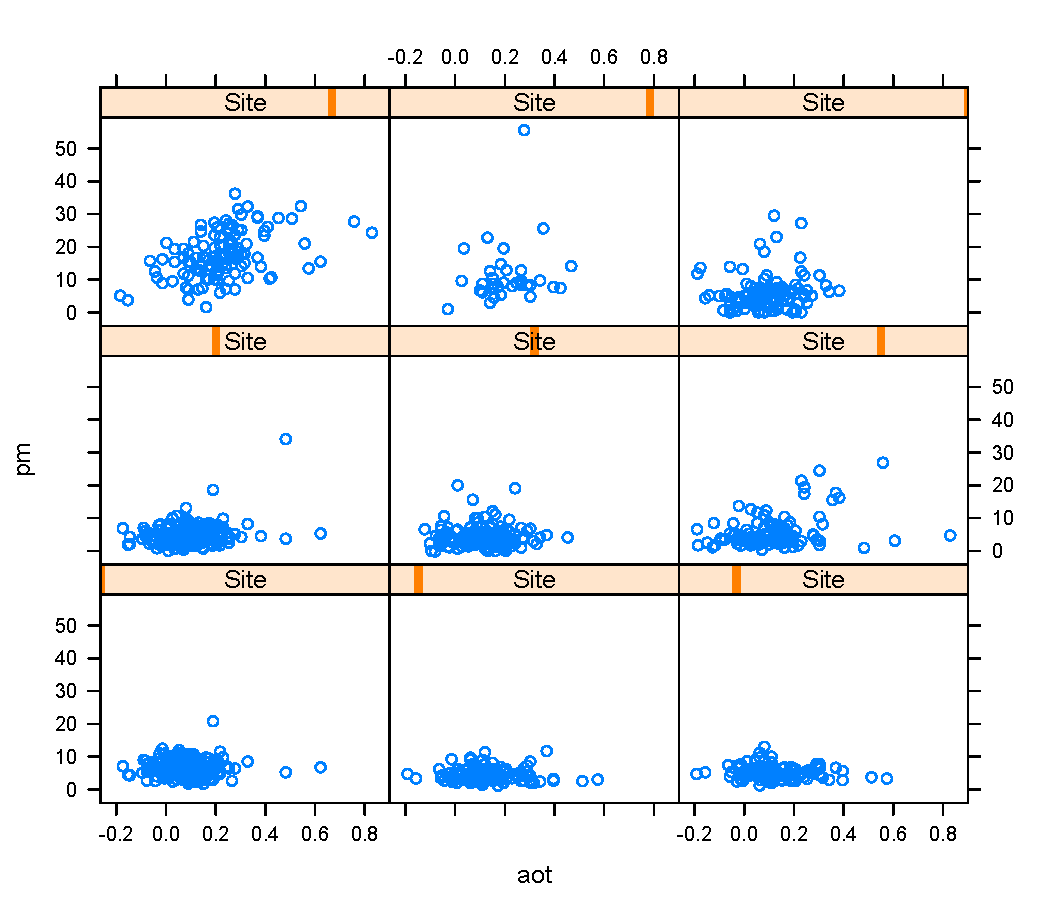
\includegraphics[width=\linewidth]{1.pdf}
\caption{PM vs. AOD for each Hawaii site}
\label{fig3.4}
\end{figure}

Similarly, we can see from the above plot that the relationships between AOD and PM2.5 are different for different sites. Like what we did for sites close to the west coast, we consider building different models for each site to find the relationships.



Give enough details so that readers can duplicate your experiments.

\begin{itemize}
\item Describe the precise purpose of the experiments, and what they 
are supposed to show.

\item Describe and justify your test data, and any assumptions you made to 
simplify the problem.

\item Describe the software you used, and the 
parameter values you selected.

\item 
For every figure, describe the meaning and units of the coordinate axes, 
and what is being plotted.

\item Describe the conclusions you can draw from your experiments
\end{itemize}

\section{Summary and Future Work}
\begin{itemize}
\item Briefly summarize your contributions, and their possible
impact on the field (but don't just repeat the abstract or introduction).
\item Identify the limitations of your approach.
\item Suggest improvements for future work.
\item Outline open problems.
\end{itemize}

\begin{thebibliography}{99}

\bibitem{noaa} National Centers for Environmental Information. National Oceanic and Atmospheric Administration. Department of Commerce, n.d. Web. 23 July 2016. \textit{https://www.ncdc.noaa.gov/cdr/atmospheric/avhrr-aerosol-optical-thickness}.
\bibitem{epa} United States Environmental Protection Agency. AirData. EPA, 5 July 2016. Web. 23 July 2016. \textit{https://www3.epa.gov/airdata/}.

%http://disc.sci.gsfc.nasa.gov/giovanni/additional/users-manual/G3_manual_Chapter_19_AOT_comparison#sat_sensor

\end{thebibliography}

\end{document}
